\documentclass[12pt]{article}	% if curious, google for different types of document classes
				% a resume class also exists and makes for a nice-looking resume

\usepackage{amsmath, amssymb, amsthm}    	% need for subequations
% \pagestyle{empty} 		% use if page numbers not wanted
\usepackage{graphicx}	% use to include graphics
\usepackage{verbatim}
\usepackage{multicol}

\makeatletter
\renewcommand\section{\@startsection{section}{1}{\z@}%
                                 {-3.5ex \@plus -1ex \@minus -.2ex}%
                                 {2.3ex \@plus.2ex}%
                                 {\normalfont\large\bfseries}}
\makeatother

\title{CSE 490h Assignment 2}
\author{
Colin Scott and Bill Cauchois \\
}

%%%% Beginning of the Document %%%%
\begin{document}

\maketitle

In this assignment we extended our RPC layer to support several different types of operations in order to implement a write-back cache coherent distributed storage algorithm coordinated by a centralized manager.

\section{Cache Coherence}

Our cache coherence algorithm was based on the IVY system described in the paper we read for class. It is \emph{write-back}, meaning that writes are not immediately propagated to the rest of the system -- instead, the propagation is delayed until another peer explicitly requests access to the file. It is \emph{linearizable}, meaning that every operation is visible to the rest of the system in a consistent total ordering. By \emph{coherent cache} we mean a store of files in which repeated reads to the same files will yield the same result, unless there is a write.

We achieve these properties through the use of a \emph{centralized manager} -- a node whose job it is to process operations from \emph{clients} while ensuring that the proper invariants are preserved and keeping track of some global state.

Note that each client maintains a \emph{file table} which contains, for each file, a lock (to ensure that the client only performs one operation on a file at a time) as well as an access modifier. File access is one of \textsc{Invalid}, \textsc{ReadOnly}, or \textsc{ReadWrite}.

\subsection{Centralized Manager}

The main invariant that the centralized manager preserves is as follows. Either a file has not yet been created, in which case all clients have \textsc{Invalid} access to that file; or, the file has been created and one client has \textsc{ReadWrite} access to that file, in which case every other client has \textsc{Invalid} access; or, the file has been created and one or more clients have \textsc{ReadOnly} access to that file, in which case every other node has \textsc{Invalid} access and no one can have \textsc{ReadWrite} access.

The global state that the centralized manager maintains is as follows. In the manager's own \emph{file table}, for each file, we have an \emph{owner} and a \emph{copy set}. A file always has exactly one owner, who has either \textsc{ReadWrite} or \textsc{ReadOnly} access to that file. The copy set for a file consists of those clients who have \textsc{ReadOnly} access to the file.

\subsection{Message Types}

Several different message types are used to synchronize state between clients and the centralized manager, as well as to transmit data. In our system, communication between nodes may never occur -- all communication goes through the centralized manager.

\begin{itemize}
\item An \textsc{InvalidateRequest} may be sent from the manager to a client to tell that client to mark its access for the specified file to \textsc{Invalid}.
\item An \textsc{InvalidateConfirm} is sent from a client to the manager to indicate that it received the \textsc{InvalidateRequest} and has performed the invalidate successfully.

\item A \textsc{ReadQuery} is sent from a client to the manager when a client wants to read a file but does not have access.
\item A \textsc{ReadForward} is sent by the manager to the owner of the file (a client) when it receives a \textsc{ReadQuery} from another node.
\item A \textsc{ReadData} may be sent in two cases: when a client receives a \textsc{ReadForward} for a file to which it has access, in which case that client sends back a \textsc{ReadData} with the contents of the file; or when the server receives a \textsc{ReadData} from a client after sending that client a \textsc{ReadForward} (in response to a \textsc{ReadQuery}), it sends a \textsc{ReadData} back to the client that originated the query.
\item A \textsc{ReadConfirm} is sent by the client after it has successfully sent a \textsc{ReadQuery} and received a \textsc{ReadData} in return. The purpose of this message is to indicate to the manager that the read has completed and it can release its lock on the file.

\item A \textsc{WriteQuery} is analagous to a \textsc{ReadQuery}, except in this case we are requesting write access to the file.
\item A \textsc{WriteForward} is sent by the manager to the owner of the file when it receives a \textsc{WriteQuery} from another node. Since when we grant \textsc{ReadWrite} access to the originator of the request it is an invariant that every other client must have \textsc{Invalid} access, a \textsc{WriteQuery} is also an implicit invalidate.
\item A \textsc{WriteData} may be sent in two cases, analagous to \textsc{ReadData}: by the manager in response to a \textsc{WriteQuery}, or by the owner in response to a \textsc{WriteForward}.
\item A \textsc{WriteConfirm} is sent by the client after it has successfully sent a \textsc{WriteQuery} and received a \textsc{WriteData} in return. The purpose of this message is to indicate to the manager that the write has completed and it can release its lock on the file.
\end{itemize}

Message types we used not from the IVY paper include:

\begin{itemize}
\item A \textsc{CreateRequest} is sent by the client to create a file.
\item A \textsc{CreateConfirm} is sent by the manager to indicate to a client that its create request has succeeded.
\item A \textsc{DeleteRequest} is sent by the client to delete a file.
\item A \textsc{DeleteConfirm} is sent by the manager to indicate to a client that its delete request has succeeded.
\end{itemize}

\subsection{Local Operations}

It bears mentioning that after a client has received a copy of a file from the manager, it writes that file to disk. Subsequent reads and writes will use the local copy of the file instead of invoking remote procedures, for efficiency's sake (as long as the client has the proper access).

\subsection{Manager as a Client}

Note also that the manager can act as a client. That is, it can perform every read/write operation that a client can perform. However, the manager does not keep a "master copy" of the cache. When it needs to read or write a file, it must send a \textsc{WriteForward} or a \textsc{ReadForward}. An optimization is that the manager does not first send a \textsc{WriteQuery} or a \textsc{ReadQuery} to itself -- in every case where a client would have to communicate with the manager, the manager (acting as a client) can eliminate the middleman.

\subsection{Example Scenarios}

We present several examples to illustrate the functioning of our system. Assume for each example that 3 nodes have been started -- node 0 is the manager, and nodes 1 and 2 are clients.

\begin{center} \textbf{Example 1} \end{center}

\begin{tabular}{p{1.5in}|p{3.3in}}
\emph{Action} & \emph{Explanation} \\
\texttt{1 create foo.txt} & Client 1 sends a \textsc{CreateRequest} to the manager, who responds with a \textsc{CreateConfirm}. In the case of a create, the client that initiated the create is set to the owner and receives read-write access. \\
\\
\texttt{1 get foo.txt} & Client 1 tries to read from foo.txt, and finds that it already has read-write access. Therefore it reads (the empty string) from its local cache on the filesystem and returns immediately. \\
\\
\texttt{2 get foo.txt} & Client 2 tries to read from foo.txt. Since it does not have a local copy (its access is set to \textsc{Invalid}), it must send a \textsc{ReadQuery} to the manager, which sends a \textsc{ReadForward} to client 1 (the owner of foo.txt). When client 1 receives this \textsc{ReadForward}, it forwards the contents of foo.txt using a \textsc{ReadData} message. The manager receives this message and sends it back to client 2. \\
\end{tabular}

\begin{center} \textbf{Example 2} \end{center}

\begin{tabular}{p{1.7in}|p{3.3in}}
\emph{Action} & \emph{Explanation} \\
\texttt{1 create foo.txt} & Client 1 creates foo.txt, as before. \\
\texttt{1 put foo.txt hello} & Client 1 tries to write to foo.txt, and finds that it has write access. Therefore, the operation completes locally with no external communication. \\
\texttt{2 get foo.txt} & Client 2 tries to read foo.txt, and finds that it has no access -- so it sends a \textsc{ReadQuery} to the manager, who sends a \textsc{ReadForward} to client 1 (the owner). The \textsc{ReadData} messages are propagated back and two other things happen: client 1 changes its access from \textsc{ReadWrite} to \textsc{ReadOnly} (since it is no longer the sole owner), and the manager adds client 2 to the copy set for foo.txt. Now client 2 has \textsc{ReadOnly} access. \\
\texttt{2 put foo.txt bye} & When client 2 tries to write to foo.txt, it must send a \textsc{WriteQuery} to the manager since it only has \textsc{ReadOnly} access. The manager, upon receiving the \textsc{WriteQuery}, invalidates foo.txt for every member of the copy set. Then it sends a \textsc{WriteForward} to the owner of the file (client 1) who responds with a \textsc{WriteData} that is then forwarded to client 2, who now performs the write locally. \\
\end{tabular}

\pagebreak

\begin{center} \textbf{Example 3} \end{center}

\begin{tabular}{p{1.7in}|p{3.3in}}
\emph{Action} & \emph{Explanation} \\
\texttt{1 create foo.txt} & Client 1 creates foo.txt, as before. \\
\texttt{2 put foo.txt hello} & Client 2 tries to write to foo.txt and finds that it has no access. Therefore it sends a \textsc{WriteQuery} to the manager which results in a \textsc{WriteForward} being sent to client 1 (the owner). The manager invalidates 1's copy of foo.txt and forwards the \textsc{WriteData} to 2, who then performs a local write. \\
\texttt{0 get foo.txt} & This case is slightly different because the ``client'' is the manager. Where a normal client would have to send a \textsc{ReadQuery}, the manager can directly send a \textsc{ReadForward} to the owner of foo.txt (which is now client 2). \\
\texttt{0 put foo.txt bye} & Again, the manager can omit sending a \textsc{WriteQuery} since it knows the owner. So the manager first invalidates the copy set of foo.txt, then sends a \textsc{WriteForward} to the owner of foo.txt (still 2), and, after receiving a \textsc{WriteData}, performs the local write. \\
\end{tabular}

\subsection{Major Differences from IVY}

There are several differences between our implementation and the cache coherence algorithm described in the IVY paper.

Perhaps the biggest difference is the addition of several new message types to support create and delete operations. The IVY protocol was for virtual memory systems, so it could assume that pages were allocated across all machines. However, since we are dealing with a file cache we must handle the creation and deletion of files. Creating a file is simple -- the client sends a \textsc{CreateRequest} to the manager, who then sets the owner of the file to that client and responds with \textsc{CreateConfirm}. Deletions are slightly more complicated, as the manager must send an \textsc{InvalidateRequest} to every member of the copy set to ensure that no one can read the file after it has been deleted.

We also simplified the ``improved centralized manager'' algorithm in the paper so that all communication happens through the server. In IVY, peers may communicate with each other for increased efficiency. In our system, peers only communicate by sending messages to the server, which may then be forwarded on to other peers.

\section{Changes to the RPC Layer}

We made several changes to the RPC layer for this assignment. We used the RPC layer exclusively to transmit messages used by the cache coherence protocol.

The biggest change was our switch to Protocol Buffers. We decided that instead of rolling our own encoding for remote procedure calls, we would use Google's Protocol Buffer library to serialize and deserialize packets. Our message types are all defined in \texttt{proj/RPCProtos.proto}.

The basis of our new RPC encoding is the \texttt{RPCEnvelope} message type, which encapsulates the type of the call, the call ID (a new field), the error code (if an error occurred), and a variable-length sequence of bytes (the "payload", another message encoded with protobuffers).

Another addition is the call ID field. The RPC client assigns every outgoing call an integer identifier (by simply incrementing it each time) and when the RPC server sends its result, it attaches that same call ID. This is used to associate calls with their results (using a HashMap in \texttt{RPCClient}), and is integral to the new handle mechanism, which is covered in the next section.

\section{New Abstractions}

We implemented several novel abstractions which make it easier (we hope) to deal with the asynchronous, callback-oriented nature of our code within the simulator framework.

\subsection{Handles}

A handle represents a "promise" for a computation that has yet to be completed. Handles are parameterized on their result type.

For the calee, using a handle is a simple as creating one inside your function and returning it. Then, call \texttt{completedSuccess} with the result value when your computation has completed -- or call \texttt{completedError} with an error code.

For the caller, using a handle involves registering a listener on returned handle. When the computation completes, your listener will be activated.

Handles allow us to effectively utilize delayed (as by the network) computations.

\subsection{Locks}

Locks are used to provide exclusive access to a resource. When acquiring a lock, you provide a callback function to be executed as soon as the lock is free. If the lock is already free, your callback is executed immediately. But if the lock has been acquired by someone else, your callback is queued until the lock is available. After you've finished using the resource, you must explicitly call \texttt{release()} inside your callback to release the lock.

\pagebreak

\section{States and Synoptic Analysis}

We drew a state diagram to model the behavior of our system, and we also analyzed its behavior using Synoptic.

Modeling the behavior at the client involves a simple set of three states, representing the different types of access that a client can have to a file, with arrows between them corresponding to different message types. Unfortunately, we weren't sure how to model the behavior of the server using a state diagram since (except where it acts like a client) the state that it has (owner and copyset) is not finite and discrete.

Our state diagram for the client was this:

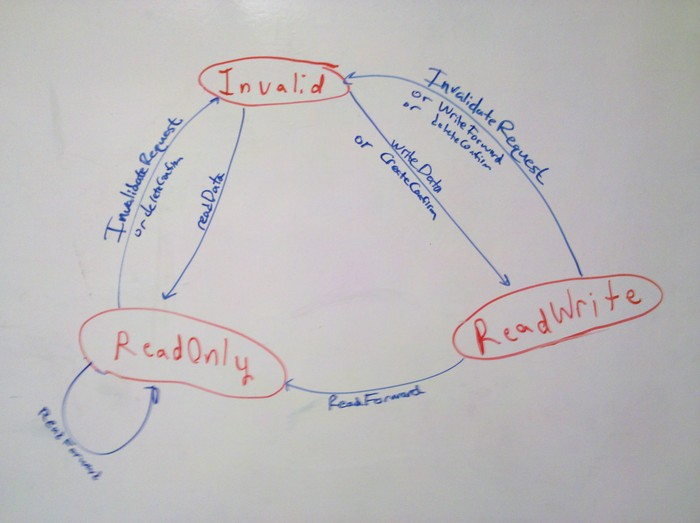
\includegraphics[width=400px]{drawn_diagram_min.jpg}

Our state diagram as a result of running synoptic on our logs was this:

\begin{center} 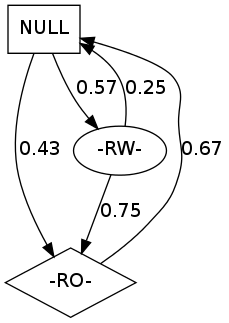
\includegraphics[width=130px]{good_synoptic_out.png} \end{center}

As you can see, the two diagrams roughly correspond. Although the labels in the second diagram are not labeled, we can see the correspondence by considering the number of incoming and outgoing edges for each ``vertex". The read only state has two incoming edges and one outgoing edge (to invalid) in each diagram. The read write state has two outgoing edges and one incoming edge (from invalid) in each diagram. The invalid state has outgoing and incoming edges to both read write and read only.

Although we were supposed to use Synoptic before we debugged, we didn't get to that part of the project until after we had fixed most of the major bugs. Therefore we cannot provide a ``before'' Synoptic diagram to complement our ``after''. However, we can confidently say that Synoptic helped confirm the correct behavior of our program, and certainly made us feel better about our code.\footnote{Thanks Ivan!}

\end{document}
